\documentclass{article}

\usepackage{tikz}
\usetikzlibrary{arrows, decorations, backgrounds, positioning, shapes.misc}

\begin{document}
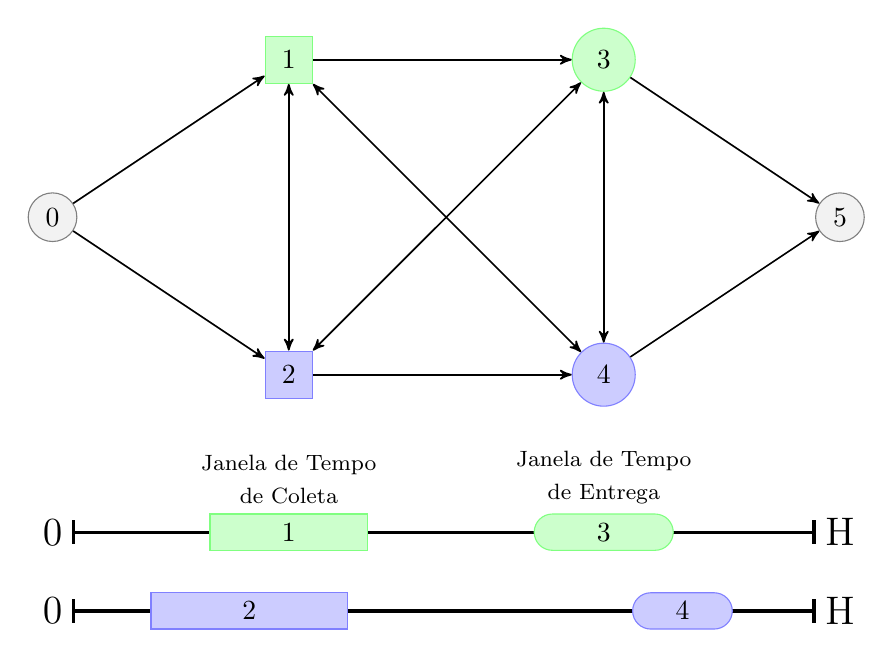
\begin{tikzpicture}
  [pickup/.style={rectangle,minimum size=6mm},
   delivery/.style={circle,minimum size=8mm},
   request1/.style={draw=green!50,fill=green!20},
   request2/.style={draw=blue!50,fill=blue!20},
   garage/.style={circle,minimum size=6mm, draw=black!50,fill=black!5},
   pre/.style={<-,>=stealth',semithick},
   duo/.style={<->,>=stealth',semithick},
   pickuptw/.style={rectangle, minimum width=20mm, minimum height=4mm},
   deliverytw/.style={rounded rectangle, minimum width=20mm, 
                      minimum height=4mm},
   timeline/.style={|-|,very thick}]

   % Grafo 
  \node (garage1) at (-5, 0) [garage] {0};
  \node (pickup1) at (-2, 2) [pickup, request1] {1}
    edge [pre] (garage1);
  \node (pickup2) at (-2,-2) [pickup, request2] {2}
    edge [pre]  (garage1)
    edge [duo] (pickup1);
  \node (delivery1) at ( 2, 2) [delivery, request1] {3}
    edge [pre]  (pickup1)
    edge [duo] (pickup2);
  \node (delivery2) at ( 2,-2) [delivery, request2] {4}
    edge [duo] (pickup1)
    edge [pre]  (pickup2)
    edge [duo] (delivery1);
  \node (garage2) at ( 5, 0) [garage] {5}
    edge [pre]  (delivery1)
    edge [pre]  (delivery2);

  % Linha de tempo
  \node (start) at (-5, -4) {\Large 0};
  \node (end) at (5, -4) {\Large H}
    edge [timeline] (start);

  % Janelas de tempo
  \node (pickup1tw) at (-2, -4) [pickuptw, request1] {1};
  \node [above, align=center] at (pickup1tw.north) 
      {\footnotesize Janela de Tempo\\ 
       \footnotesize de Coleta};
  \node (delivery1tw) at (2, -4) [deliverytw, request1] {3};
  \node [above, align=center] at (delivery1tw.north) 
      {\footnotesize Janela de Tempo\\ 
       \footnotesize de Entrega};

  % Linha de tempo
  \node (start) at (-5, -5) {\Large 0};
  \node (end) at (5, -5) {\Large H}
    edge [timeline] (start);

  % Janelas de tempo
  \node (pickup1tw) at (-2.5, -5) [pickuptw,request2,minimum width=25mm] {2};
  \node [above, align=center] at (pickup1tw.north) {};
  \node (delivery1tw) at (3, -5) [deliverytw,request2,minimum width=15mm] {4};
  \node [above, align=center] at (delivery1tw.north) {};

\end{tikzpicture}
\end{document}
